\section{Background}
\label{sec:background}

This section describes the base tensor core that FourShadow extends (Section~\ref{sec:bg_tcu}) and the concepts it depends on: the SIMT hierarchy and the threads per warp (Section~\ref{sec:bg_hierarchy}), the issue width and warpgroups (Section~\ref{sec:bg_issue}), and shared memory with DXA, the engine that fills it (Section~\ref{sec:bg_smem}).

\subsection{SIMT Hierarchy and Threads per Warp}
\label{sec:bg_hierarchy}

The base tensor core is built into Vortex~\cite{vortex}, an open-source RISC-V GPU. A Vortex processor is organized as clusters of cores; inside a cluster, a socket groups the cores that share first-level caches. The number of clusters, the cores per cluster and the cores per socket are compile-time parameters.

Each core is a SIMT pipeline that runs $\mathit{NW}$ warps. A warp is a group of $\mathit{NT}$ threads that execute the same instruction on $\mathit{NT}$ lanes of the datapath, so the threads per warp ($\mathit{NT}$) set the width of every per-thread structure: the register file holds $\mathit{NT}$ entries per architectural register, and the load/store unit has $\mathit{NT}$ lanes. Both $\mathit{NW}$ and $\mathit{NT}$ are compile-time parameters.

\subsection{Base Tensor Core}
\label{sec:bg_tcu}

As shown in Figure~\ref{fig:figure_integration}, the FourShadow Tensor Core Unit (TCU) is integrated into the Vortex GPGPU architecture as a standard functional unit alongside the ALU, FPU, LSU, and SFU within each core's execute stage. The TCU shares all essential SIMT core frontend components--- warp scheduler, scoreboard, fetch, decode --- as well as the memory hierarchy including Register Files, Shared Memory and L1 and L2 caches. Inside the TCU a grid of Fused Dot Product (FEDP) units serve as the core compute engine for the MMA instructions. Each FEDP unit computes one element of $D$ as in Equation~(\ref{eq:fedp}).

\textbf{Full-configurability:}
The FourShadow TCU is fully parameterizable by warp size (Number of Threads ($\mathit{NT}$)), as a single compile-time parameter that determines register file capacity, tile dimensions, FEDP unit count, and sub-block packing as derived in (Figure~\ref{fig:tiling_equations}). This exposes architectural exploration opportunities unavailable on fixed-warp proprietary designs. Below, we detail the matrix-to-register mapping, FEDP scheduling, and mixed-precision datapath adaptation.

\begin{figure}[ht]
\small
\hrule
\vspace{3pt}
{\raggedright\textit{Given:}\ $M,\,N,\,K$} \\
{\raggedright $\mathit{Number of Threads (NT)=\{2, 4, 8, 16, 32\}}$ } \\ 
{\raggedright $\mathit{Number of Registers (NR)}{=}8$\par}
\centering\textbf{\textsc{Tile (per-warp work chunk)}}
\begin{flalign}
&\mathit{tile\_cap} = \mathit{NT} \!\times\! \mathit{NR},\quad
\ell_g = \lfloor\log_2(\mathit{tile\_cap})\rfloor & \\
&\mathit{xtileM} = 2^{\,\ell_g - \lfloor\ell_g/2\rfloor},\quad
\mathit{xtileN} = 2^{\,\lfloor\ell_g/2\rfloor} & \\
&\mathit{xtileK} = \tfrac{\mathit{tile\_cap}}{\max(\mathit{xtileM},\,\mathit{xtileN})} & \\
&\mathit{tileK} = \mathit{xtileK}\!\times\!\tfrac{4}{\mathrm{sizeof}(\texttt{input\_dtype})} &
\end{flalign}
\noindent\textbf{\textsc{Block (one micro-op)}}
\begin{flalign}
&\mathit{block\_cap} = \mathit{NT},\quad
\ell_b = \lfloor\log_2(\mathit{block\_cap})\rfloor & \\
&\mathit{tcM} = 2^{\,\ell_b - \lfloor\ell_b/2\rfloor},\;\;
\mathit{tcN} = 2^{\,\lfloor\ell_b/2\rfloor},\;\;
\mathit{tcK} = \tfrac{\mathit{block\_cap}}{\max(\mathit{tcM},\,\mathit{tcN})} &
\end{flalign}
\hrule
\vspace{3pt}
\noindent\textbf{\textsc{Steps (micro-ops per tile)}}
\begin{flalign}
&m_{\mathrm{steps}} = \tfrac{\mathit{xtileM}}{\mathit{tcM}},\quad
n_{\mathrm{steps}} = \tfrac{\mathit{xtileN}}{\mathit{tcN}},\quad
k_{\mathrm{steps}} = \tfrac{\mathit{xtileK}}{\mathit{tcK}} &
\end{flalign}
\noindent\textbf{\textsc{Grid (tiles covering full matrix)}}
\begin{flalign}
&\mathit{num\_tiles}_M = \left\lceil\tfrac{M}{\mathit{xtileM}}\right\rceil,\quad
\mathit{num\_tiles}_N = \left\lceil\tfrac{N}{\mathit{xtileN}}\right\rceil & \\
&\mathit{num\_tiles}_K = \left\lceil\tfrac{K}{\mathit{tileK}}\right\rceil &
\end{flalign}
\hrule
\vspace{3pt}
{\centering\textbf{\textsc{micro-ops per \texttt{mma\_sync}}}\par}
{\raggedright
\noindent\hspace{0.5em}\textbf{for} $\;0$ \textbf{to} $k_{\mathrm{steps}}{-}1$:\\
\hspace{2em}\textbf{for} $\;0$ \textbf{to} $m_{\mathrm{steps}}{-}1$:\\
\hspace{3.5em}\textbf{for} $\;0$ \textbf{to} $n_{\mathrm{steps}}{-}1$:\\
\hspace{5em}one micro-op: $\mathit{tcM}{\times}\mathit{tcN}{\times}\mathit{tcK}$ dot-product
\par}
\hrule
\caption{Tensor-core tiling and micro-op decomposition derived from thread count~$\mathit{NT}$ and register budget~$\mathit{NR}$.}
\label{fig:tiling_equations}
\end{figure}

\textbf{Matrix-Register Mapping:}
Vortex's RV32 ISA provides 32 floating-point registers per thread. Among 32, FourShadow utilizes 24 registers equally partitioned into three groups of $\mathit{NR}{=}8$ registers for matrices $A$, $B$ and $C/D$. Each register corresponds to $\mathit{NT}$ physical 32-bit entries, so the total per-matrix capacity scales with $\mathit{NT}$. Because this register count is a hard architectural limit, the original matrix must be decomposed into tiles that fit entirely within the available register space.

\begin{figure}[ht]
    \centering
    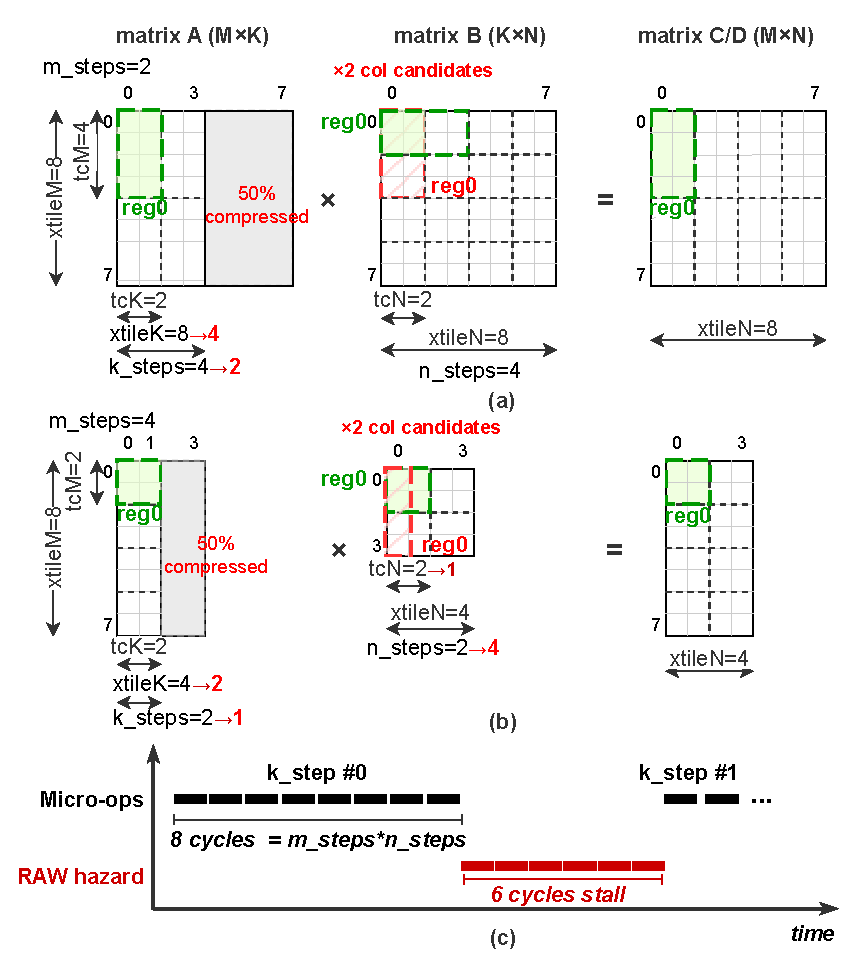
\includegraphics[width=\columnwidth]{hpca2027-latex-template/fig/tcu_matrix_register_mapping_sparse_v4.pdf}
    \caption{Matrix-to-register mapping and tiling for (a) 8-thread.(b) 4-thread configurations. (green : dense, red : sparse) (c) RAW hazard within the micro-ops} 
    \label{fig:figure_register_mapping}
\end{figure}

Figure~\ref{fig:figure_register_mapping}(a) illustrates the resulting mapping for $\mathit{NT}{=}8$, where $\mathit{xtileM}{=}\mathit{xtileN}{=}\mathit{xtileK}{=}8$; the green-shaded regions show how \texttt{reg0}--\allowbreak\texttt{reg7} tile across the matrix dimensions for $A$, $B$, and $C$/$D$. Figure~\ref{fig:figure_register_mapping}(b) shows the $\mathit{NT}{=}4$ case, where the halved thread count shrinks the tile to $8{\times}4{\times}4$ and matrix~$B$ utilizes only half its register budget.

\textbf{Thread-FEDP Mapping:}
Each TCU core contains a $\mathit{tcM}{\times}\mathit{tcN}$ grid of $\mathit{NT}$ number of FEDP unit instantiations, each producing one element of~$D$.

In Figure~\ref{fig:figure_register_mapping}(a) with $\mathit{NT}{=}8$, the green-shaded block within \texttt{reg0} of matrix~$B$ occupies only half the register width---this is an \emph{asymmetric} configuration where two adjacent $B$ blocks pack into one register. In contrast, Figure~\ref{fig:figure_register_mapping}(b) with $\mathit{NT}{=}4$ shows the \emph{symmetric} case: the green-shaded $B$ block fills \texttt{reg0} entirely, yielding a one-to-one register-to-block correspondence. Among the supported thread counts, $\mathit{NT}{\in}\{2,\allowbreak 8,\allowbreak 32\}$ produce asymmetric configurations, while $\mathit{NT}{\in}\{4,16\}$ produce symmetric ones.

The full tile is covered by iterating micro-ops in the order shown in Figure~\ref{fig:tiling_equations}: $n$ innermost, $m$ middle, $k$ outermost. As annotated in Figure~\ref{fig:figure_register_mapping}, the $\mathit{NT}{=}8$ tile totals $4{\times}2{\times}4{=}32$ micro-ops, while the $\mathit{NT}{=}4$ tile totals $2{\times}4{\times}2{=}16$. 

Some micro-architectural implications that FourShadow can explore are discussed as follows.
Figure~\ref{fig:tiling_equations} shows that m\_steps*n\_steps is fixed
as 8 regardless of NT. This fixed product of eight determines the
accumulator reuse distance: each $(m,n)$ accumulator register is
re-read exactly $m\_steps \times n\_steps = 8$ micro-instructions after
it was written, at the next $k$-iteration. However, the TCU pipeline
commits the result after 14 cycles, so the scoreboard stalls the
dependent read for approximately $14{-}8{=}6$ cycles at every
$k$-loop boundary---a structural RAW
hazard(Figure~\ref{fig:figure_register_mapping}(c)) that FourShadow's
multi-warp scheduler can partially hide by interleaving independent
warps into the gap.

A second class of pipeline stall arises from the register file itself.
At each tensor-core micro-op, the operand-collection unit concurrently
fetches three source registers---one each from matrices $A$, $B$, and
$C/D$---from a physical register file partitioned into four banks
indexed by the low two bits of the register number. The naive placement
($C/D$ at \texttt{f0..f7}, $A$ at \texttt{f10..f17}, $B$ at
\texttt{f24..f31}) leaves $B$ and $C/D$ on the same cyclic bank
residue, forcing a one-cycle stall whenever their register offsets
match modulo four. We eliminate this by relocating $B$ from
\texttt{f24..f31} to \texttt{f21..f28}, shifting its bank pattern by
one position so that $A$, $B$, and $C/D$ each occupy a distinct cyclic
shift modulo four and all three operands are served in a single cycle.
This reduces register-file bank-conflict stalls by up to 24~percentage
points.

\textbf{FEDP Microarchitecture \& Datatypes:}\label{para:datatypes-fedp} The FourShadow TCU is realized using the highly configurable 4-cycle latency Ten-Four~\cite{rout2026tenfouropensourcefuseddot} mixed-precision FEDP microarchitecture. It consists of four pipeline stages: multiply $\rightarrow$ align $\rightarrow$ accumulate $\rightarrow$ normalize-and-round, producing a fully fused result without intermediate rounding. We support low-precision multiplication in TF32, FP16, BF16, FP8(E4M3), BF8(E5M2), INT8, and INT4 with higher-precision accumulation in FP32 and INT32 respectively. Ten-Four's RTL can be configured at compile-time to selectively enable or disable individual input formats, and FourShadow inherits this configurability directly. For example, a researcher studying mixed-precision training schemes combining BF16 forward passes with FP8 gradient accumulation can enable exactly those two formats only, producing a leaner datapath tuned to the workload.

The effective reduction length of each FEDP invocation scales with the bitwidth of the active input format, since narrower types pack more elements into each 32-bit register slot. For a tile of fixed logical dimension \texttt{tileK}, FP16 and BF16 pack two elements per 32-bit slot, doubling the reduction length to $2 \times \texttt{tileK}$; FP8, BF8, and INT8 pack four elements, yielding $4 \times \texttt{tileK}$. For instance, when $NT=32$ the WMMA core dimensions are \texttt{8x4x4} in the baseline 32-bit (and TF32) case, \texttt{8x4x8} for FP16/BF16, and \texttt{8x4x16} for FP8/BF8/INT8. This register-packing scheme reduces memory bandwidth and footprint alongside compute density.

\subsection{Issue Width and Warpgroups}
\label{sec:bg_issue}

The issue width is the number of warps from which a core issues an instruction in the same cycle. The issue stage is divided into that many issue slots, and the warps are interleaved over the slots by warp index, so each slot serves $\mathit{NW}$ divided by the issue width warps. An issue width of one issues from a single warp per cycle.

The tensor core scales with the issue width: the core instantiates one tensor block, a complete $\mathit{NT}$-unit FEDP grid, per issue slot. The warps that issue together, one from each slot, form a \emph{warpgroup}; the size of a warpgroup therefore equals the issue width, and the tensor blocks of a core can serve all warps of one warpgroup in the same cycle. On NVIDIA GPUs a warp has 32 threads and a warp group has four warps~\cite{luo2025dissectingnvidiahopperarchitecture}; that point corresponds to $\mathit{NT}{=}32$ and an issue width of four here. The instruction that makes the warps of a warpgroup cooperate on one matrix operation is part of our design (Section~\ref{sec:design_wgmma}).

\subsection{Shared Memory and DXA}
\label{sec:bg_smem}

Shared memory is a scratchpad private to each core and shared by the warps that run on it. It is divided into $\mathit{NT}$ banks, one per thread of a warp, and consecutive words fall into consecutive banks, so the $\mathit{NT}$ threads of a warp read or write $\mathit{NT}$ consecutive words through $\mathit{NT}$ different banks. Each bank holds 2\,KB with a floor of 8\,KB for the whole memory, which gives 8, 16, 32 and 64\,KB for $\mathit{NT}$ of 4, 8, 16 and 32.

A kernel fills shared memory from global memory either with ordinary per-thread loads and stores or through DXA. DXA is Vortex's counterpart of the Tensor Memory Accelerator of NVIDIA Hopper~\cite{nvidia2022hopper}: a warp issues one instruction that names a pre-programmed descriptor of a tile, and an engine shared by the cores of a socket copies that tile from global memory into shared memory asynchronously while the warp continues with other work. The warp-group tensor core of Section~\ref{sec:design_wgmma} reads its operands from shared memory.

\section{Motivation}
\label{sec:motivation}

\begin{table*}[t]
\centering
\caption{Comparison of GPU tensor-core architectures, simulators and related research.}
\label{tab:related_work_comparison}
\renewcommand{\arraystretch}{0.9}
\resizebox{\textwidth}{!}{%
\begin{tabular}{p{2.4cm} p{2.4cm} p{3.6cm} p{2.6cm} p{2.2cm} p{1.5cm} c c}
\toprule
\textbf{Paper} &
\textbf{Simulation} &
\textbf{Data Types} &
\textbf{Thread Config.} &
\textbf{Sparsity} &
\textbf{TC Style} &
\makecell{\textbf{Low Latency}\\\textbf{Dot Product}} &
\makecell{\textbf{Open}\\\textbf{Source}} \\
\midrule
\rowcolor{blue!8}
\textbf{FourShadow (Ours)}
  & Cycle-sim, RTL
  & TF32, FP16/8, BF16/8, \newline INT8/4
  & 2, 4, 8, 16, 32
  & 2:4 structured
  & SIMT
  & Fused (RTL)
  & \cyes \\
\midrule
\textbf{Virgo}~\cite{kim2025virgo}
  & Cycle-sim, RTL
  & INT8/32
  & Fixed 32
  & \cno
  & Systolic
  & Discrete
  & \cyes \\
\midrule
\textbf{CoopWarp}~\cite{nada2025cooperative}
  & Cycle-sim
  & FP8, FP16, BF16, FP32
  & 4, 8, 16, 32
  & \cno
  & SIMT
  & Discrete
  & \cyes \\
\midrule
\textbf{RM-STC}~\cite{huang2023rmstc}
  & Cycle-sim
  & FP16, INT8
  & Fixed 32
  & Any degree
  & SIMT
  & Discrete
  & \cno \\
\midrule
\textbf{VEGETA}~\cite{jeong2023vegeta}
  & Cycle-sim, RTL
  & BF16, FP32
  & No SIMT
  & N:M flexible
  & Systolic
  & Discrete
  & \cno \\
\midrule
\textbf{SIMD$^2$}~\cite{zhang2022simd2}
  & HW emulation
  & FP16, INT8
  & Fixed 32
  & \cno
  & SIMT
  & Discrete
  & \cno \\
\midrule
\textbf{Accel-Sim}~\cite{accel-sim}
  & Cycle-sim
  & FP16
  & Fixed 32
  & \cno
  & SIMT
  & Fused (Sim)
  & \cyes \\
\midrule
\textbf{Sparse TC}~\cite{zhu2019sparsetensorcore}
  & Cycle-sim
  & FP16, INT8
  & Fixed 32
  & Vector N:M
  & SIMT
  & Discrete
  & \cno \\
\midrule
\textbf{GPGPU-Sim}~\cite{raihan2019modeling}
  & Cycle-sim
  & FP16/32
  & Fixed 32
  & \cno
  & Modeled
  & Fused (Sim)
  & \cyes \\
\bottomrule
\end{tabular}%
}
\end{table*}

Two facts about what is public on tensor cores motivate this work: their features are documented without their causes, which existing simulation frameworks cannot supply either (Section~\ref{sec:mot_causes}), and a commercial GPU exposes one design point (Section~\ref{sec:mot_point}).

\subsection{Tensor-Core Features Are Documented Without Their Causes}
\label{sec:mot_causes}

Vendor documents and microbenchmarking studies report what each tensor-core feature delivers. For 2:4 structured sparsity, NVIDIA states that Sparse Tensor Cores double the throughput of tensor-core operations~\cite{nvidia2020ampere}. At the level of a GEMM the speedup depends on arithmetic intensity and on the GEMM dimensions, and approaches 2$\times$ only for larger GEMMs~\cite{mishra2021acceleratingsparsedeepneural}. At the level of one instruction, sparse \texttt{mma} instructions on an H800 reach an average of 1.42$\times$ the throughput of the dense ones~\cite{luo2025dissectingnvidiahopperarchitecture}.

Warp-group MMA shows the same pattern. The instruction takes matrix $A$ either from registers (RS mode) or, like matrix $B$, from shared memory (SS mode). On the H800, the dense instruction has the same latency in both modes, whereas the sparse instruction takes 128 cycles in RS mode and 144 cycles in SS mode~\cite{luo2025dissectingnvidiahopperarchitecture}.

These sources give the outcome and leave its microarchitectural cause open. The study that measures the two modes suggests that the doubled shared-memory access demand of the sparse SS mode may be the reason~\cite{luo2025dissectingnvidiahopperarchitecture}. On a commercial GPU the operand path, the metadata path and the tensor-core array are neither observable nor changeable one at a time, so such an explanation cannot be tested there.

Existing simulation frameworks cannot supply the cause either, because they abstract the tensor core. Accel-Sim~\cite{accel-sim} gives every tensor-core instruction one latency and one initiation interval, both read from a single configuration option. A tensor-core instruction is thus represented by two numbers. Its micro-op sequence, the delivery of its operands from registers or shared memory, and its sparsity metadata are below the resolution of such a model, so the model cannot attribute a measured outcome to any one of them. GPGPU-Sim~\cite{raihan2019modeling} also models the tensor core inside a cycle-level simulator; the Accel-Sim and GPGPU-Sim rows of Table~\ref{tab:related_work_comparison} show both with the warp fixed at 32 threads and without sparsity.

\subsection{A Commercial GPU Exposes One Design Point}
\label{sec:mot_point}

A commercial GPU ships one point of the tensor-core design space: 32 threads per warp and four warps per warp group on NVIDIA GPUs~\cite{luo2025dissectingnvidiahopperarchitecture}. Microbenchmarking studies measure that point across GPU generations, instruction shapes and data types~\cite{jia2018dissectingnvidiavoltagpu, jia2019dissectingnvidiaturingt4, 9931992, luo2025dissectingnvidiahopperarchitecture}. The threads per warp and the issue width are fixed in silicon, so their interaction cannot be measured on any shipped part: the return of a wider issue width at 32 threads per warp against 16 or 4 threads per warp is one such interaction. Research platforms mostly keep this point: in the thread-configuration column of Table~\ref{tab:related_work_comparison}, every GPU platform except CoopWarp~\cite{nada2025cooperative} fixes the warp at 32 threads. A simulation framework can change the parameters that silicon fixes, but a model that represents a tensor-core instruction by one latency and one initiation interval (Section~\ref{sec:mot_causes}) has no tensor-core organization to vary together with the threads per warp and the issue width. The design points around the commercial one are therefore unmeasured, and the headroom they hold is unexplored.

\textbf{Positioning and roadmap.} FourShadow is an open, synthesizable and reconfigurable tensor-core microarchitecture on a RISC-V GPU. It obtains the causes by design-space exploration, changing one microarchitectural parameter at a time, and it is released as a framework for further tensor-core studies. No prior platform listed in Table~\ref{tab:related_work_comparison} combines configurable thread counts, the listed data types, 2:4 structured sparsity and an open RTL implementation. For the design points of Section~\ref{sec:mot_point}, Section~\ref{sec:eval_hierarchy} scales the threads per warp, the issue width and the cores per cluster. For the causes of Section~\ref{sec:mot_causes}, the warp-group tensor core is designed in Section~\ref{sec:design_wgmma} and explored in Section~\ref{sec:eval_wgmma}, and the sparse tensor core is designed in Section~\ref{sec:design_sparse} and explored in Section~\ref{sec:eval_sparse}; its causes are obtained by the comparison with a commercial GPU in Sections~\ref{sec:eval_sparse_halves} and~\ref{sec:eval_sparse_meta}. Section~\ref{sec:methodology} describes how these measurements are compared with those of a commercial GPU.
